\chapter{Mechanical Structure and Envelope}
\label{chap:mse}

The first subsystem is the \ac{MSE}. It is considered to be the foundation of the entire airship, seeing the fact that it acts as the basis which withstands all external influences and holds all the other subsystems together. This subsystem also includes the device that will be generating the lift for the entire \ac{SPA}. The fact that now an ESRANGE blimp is used, rather than a custom-made blimp (due to time constraints), has modified virtually every requirement that was defined in the preliminary design (refer to the \ac{PDR} for more information). Therefore this chapter will cover the updated requirements and constraints together with a view on the possible alternatives to overcome the problems that are currently being faced. Also the updated design and the construction phase will be presented. The reader should however bear in mind that this chapter contains only guidelines to take the firsts steps, given that the design is not finished due to the uncertainty regarding the final components.

\section{Functional and Technical Requirements}

This section will cover the updated requirements that are the consequences of the choices taken during the course of the project. The functional requirements have of course not changed, but the same cannot be said about the technical requirements.

\subsection{Functional Requirements}

The \ac{MSE} should have the following properties or be capable of the following functions.

\begin{itemize}
\item Aerodynamic stability
\item Support the solar cells, the propulsion system and the scientific payload
\item Sufficient lift to overcome the weight of the entire system
\item Low diffusivity for the balloon material
\end{itemize}

\subsection{Technical Requirements}

The previously calculated/estimated parameters have been modified to fit the constraints imposed by the new ESRANGE blimp. They are presented in Table \ref{tab:technical}.

\begin{table}[H]
\centering
\caption{Technical requirements}
\label{tab:technical}
\begin{tabular}{c c}
\hline
\textbf{Parameter} & \textbf{Value}\\ \hline
Length & $4.94\,m$\\
Diameter & $1.89\,m$\\
Volume & $15\,m^3$\\
Maximum lift mass & $2.59\,kg$\\
Maximum lift payload mass & $0.5\,kg$\\
Maximum lift structural mass & $1\,kg$\\
Maximum lift \ac{EPS} mass  & $1\,kg$\\
\hline
\end{tabular}
\end{table}

\noindent
Comparing the new available maximum lift mass provided by the blimp, it can be seen that the new total mass is half that of which was initially assumed during the \ac{PDR}. This entails that the mass budgets available for each of the subsystems have to be redistributed. For the \ac{MSE} subsystem in particular, the consequence is a complete redesign of the entire structure, dismissing the initial idea of a rigid structure. The next section explains how the design was modified, also presenting suggestions for the corresponding new structural components.

\section{Critical Design}

As was mentioned in the \ac{PDR}, the initial mechanical design of the \ac{U-SPACE} project included the development of a blimp (envelope) that accommodates the solar panels of the \ac{EPS}, the cargo bay for the \ac{ITPU} subsystem and the propelling system of the \ac{MCC} subsystem. An initial sketch of this concept is presented in Figure \ref{fig:init}. 

\pagebreak

\begin{figure}[bht]
\centering
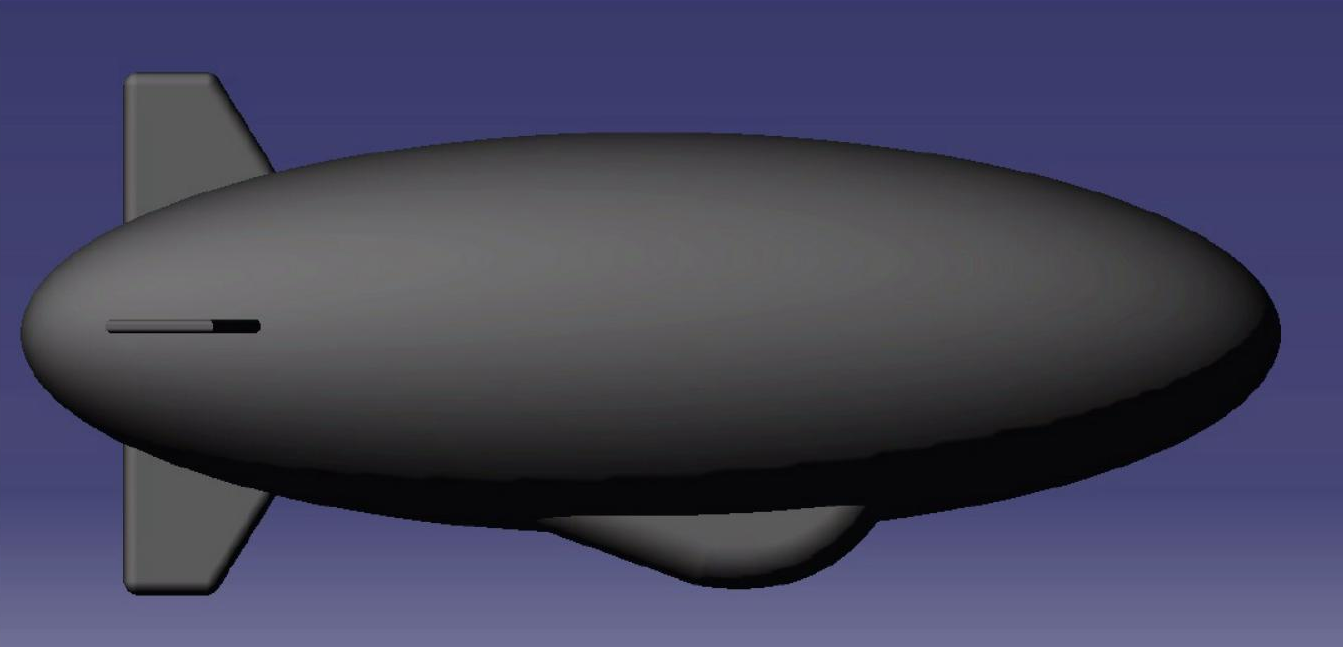
\includegraphics[scale=0.5]{figures/init.png}
\caption{Initial 3D sketch of the SPA concept}
\label{fig:init}
\end{figure}

\noindent
This simplified view of the mechanical design shows that it included the development of an envelope for the airship. The idea was to attach the solar panels on the top, mounted onto a wired mesh, with the cargo bay located at the bottom together with the propelling system.
\\
\\
However, due to new developments in the project that included the introduction of an already built blimp (envelope), the focus of the mechanical design was changed. The blimp to be used is the TIF-250 \cite{website:tif250}, shown in Figure \ref{fig:blimp}. This blimp has the capacity to lift a payload of about 2.5 kg, has a length of approximately 5 m and has a diameter (in the center) of about 1.9 m (see Table \ref{tab:technical}).

\vspace{1.0em}

\begin{figure}[bht]
\centering
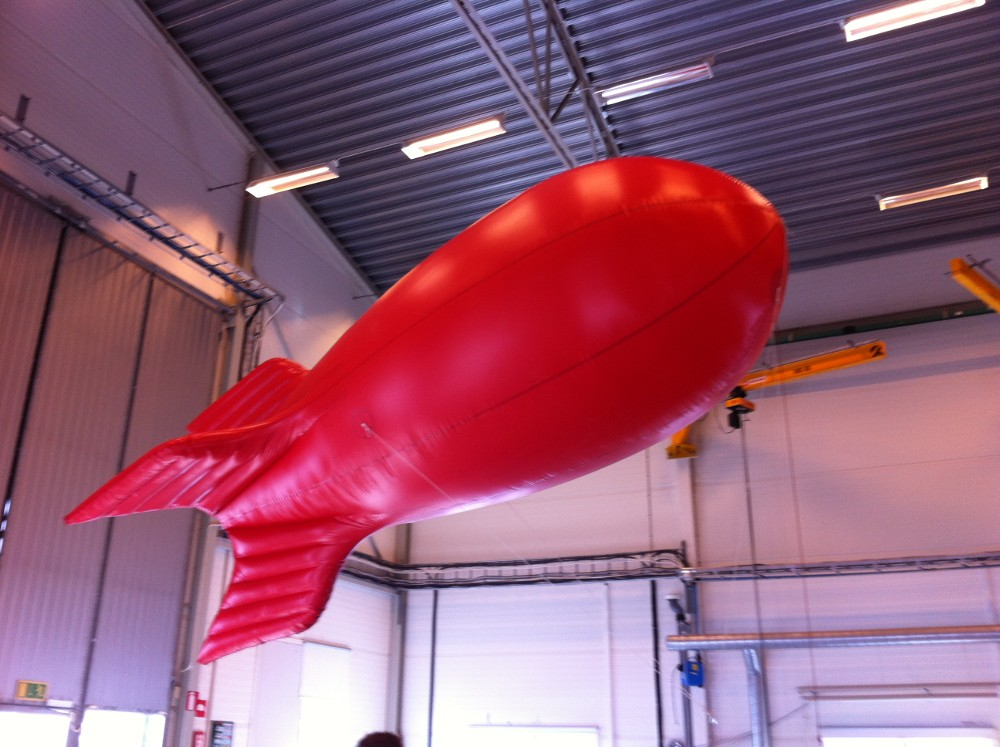
\includegraphics[width=\textwidth]{figures/blimp.jpg}
\caption{TIF-250 blimp}
\label{fig:blimp}
\end{figure}

\noindent
This blimp serves the purpose of the U-SPACE project very well, as using it would allow to focus only on the construction of the support for the \ac{EPS}, on the cargo bay for the payload and on the integration of the propelling system. However, because it is a ready-built blimp with a purpose different than the one envisioned, it is not as lightweight as required. Nevertheless, light structures will be included in the integration of all other systems to remedy this problem.

\subsection{Envelope}

As was mentioned above, the blimp to be used is already built. This blimp is normally used to accurately measure the wind direction. Nevertheless it will have to fit the purpose of the U-SPACE project, due to the lack of time to build a new envelope. The blimp itself thus functions as the envelope.  

\subsection{Cargo Bay}

The cargo bay accommodates both the payload and the electronics required for \ac{U-SPACE}. The main challenge in the construction of this cargo bay is the mass. It has to be lightweight (the maximum total mass of all structures should be less than 1 kg) but at the same time rigid enough to resist some stress during the normal operation of the airship. To achieve this functionality balsa wood reinforced with carbon fibres is used. Figures of the envisioned final cargo bay design and of the current construction status are presented in Figures \ref{fig:box} and \ref{fig:boxinit} respectively. 

\begin{figure}[th!]
\centering
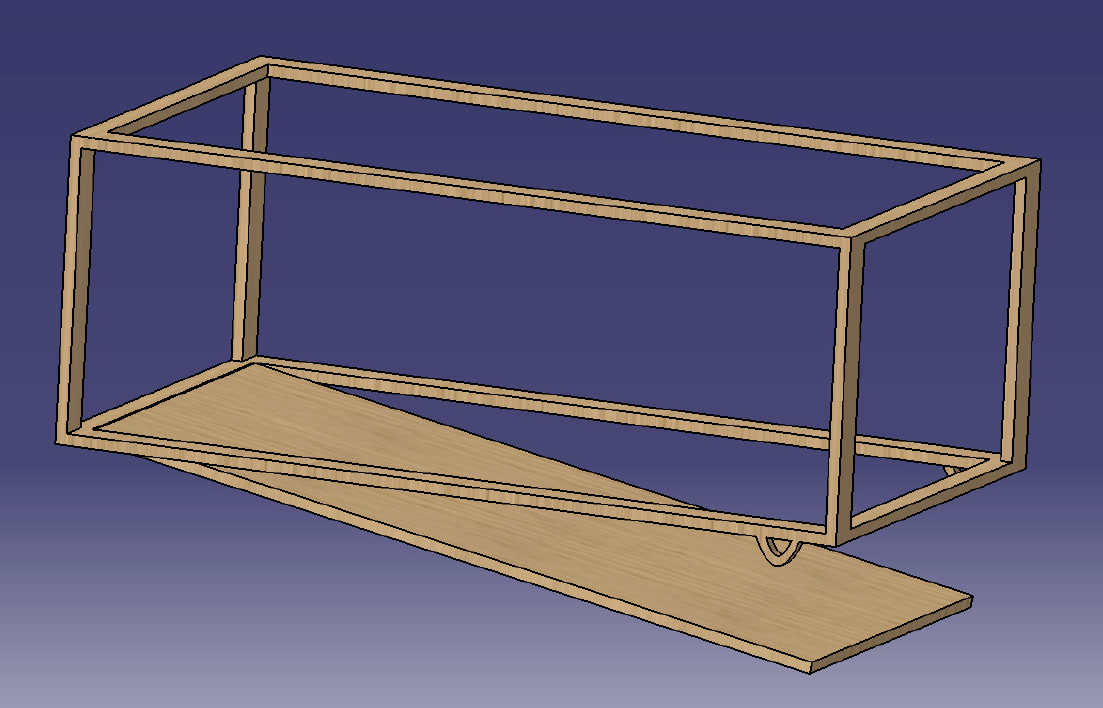
\includegraphics[scale=0.5]{figures/box.png}
\caption{3D sketch of the cargo bay} 
\label{fig:box}
\end{figure}

\begin{figure}[th!]
\centering
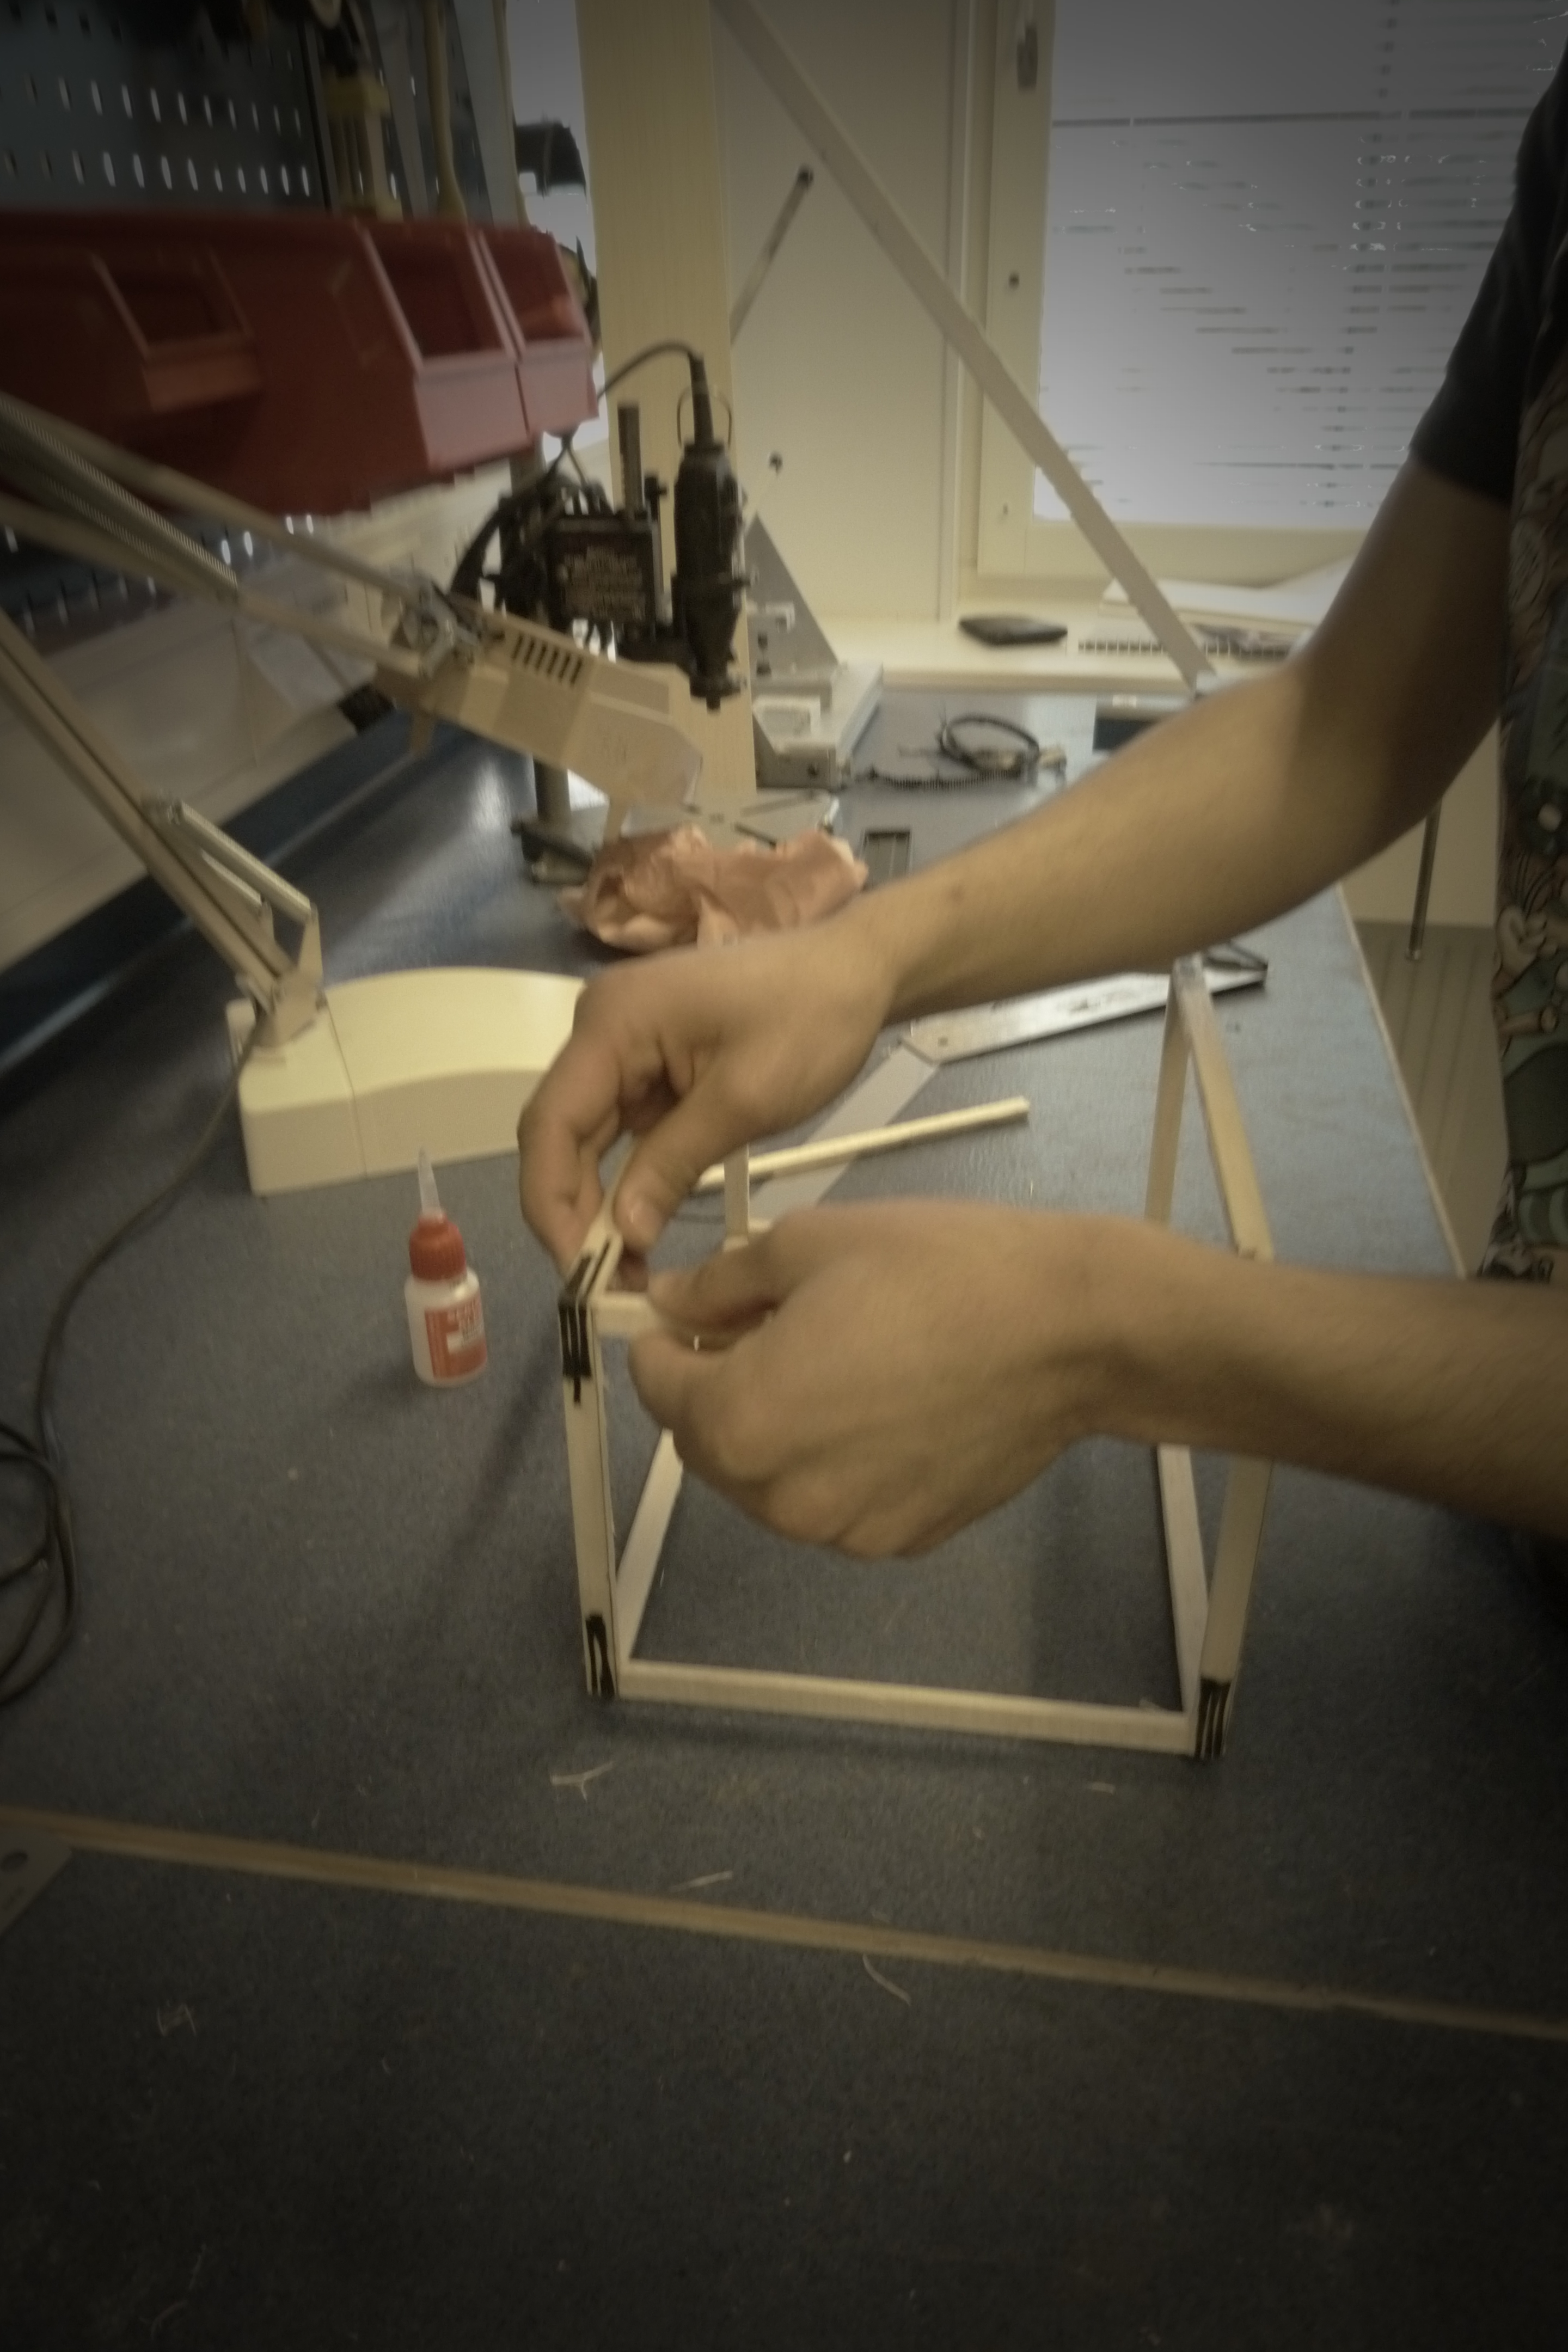
\includegraphics[scale=0.5]{figures/boxinit.jpg}
\caption{Initial construction phase of the cargo bay}
\label{fig:boxinit}
\end{figure}

\subsection{Power System}

The biggest challenge in this project is the accommodation of the power system, taking into account the maximum lift mass and the power requirements that consequently influence the solar panel quantity and mass. Because different solar panels are still being testes, it has not yet been decided how they will be mounted onto the blimp. Nevertheless, the idea is to use a lightweight wired mesh that serves as a support for the solar panels, which are attached to the wires with carbon fibre. This mesh is connected to the blimp by making use of three bands that will go around the blimp, distributing the weight along the envelope. These bands are made of fibre glass reinforced rubber tape. An idea of how the final design could look like is presented in Figure \ref{fig:mesh}.

\pagebreak

\begin{figure}[bht]
\centering
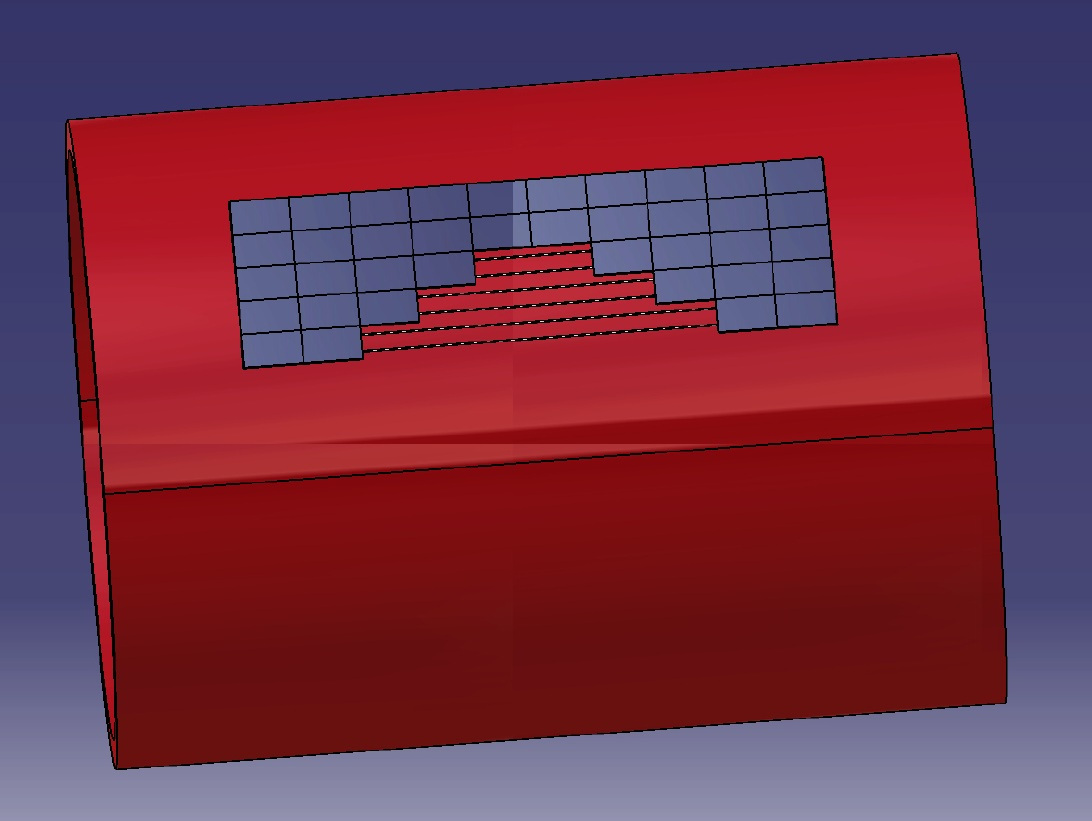
\includegraphics[scale=0.4]{figures/mesh.jpg}
\caption{3D sketch of the integration of the power system}
\label{fig:mesh}
\end{figure}

\subsection{Propelling System}

The propelling system is attached to a carbon fibre rod mounted onto the top of the cargo bay. The two motors are attached at the ends of the rod, away from the influence of the envelope and free to achieve their maximum aerodynamic capabilities. A hand sketch of this principle is shown in Figure \ref{fig:prop}.

\begin{figure}[h!]
\centering
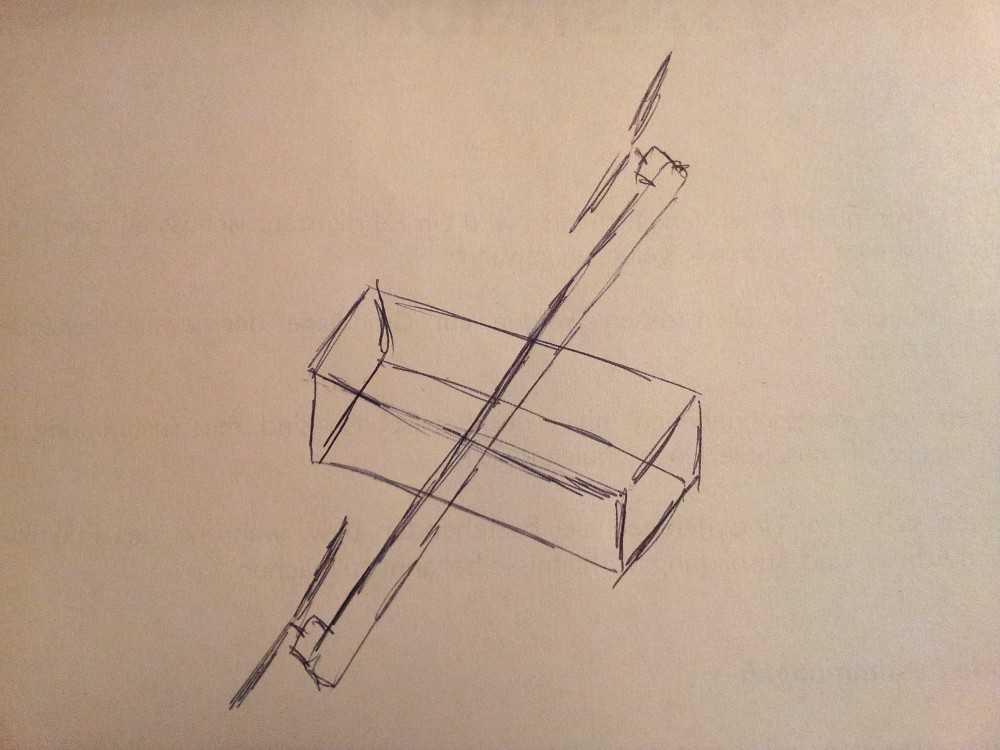
\includegraphics[scale = 0.3]{figures/prop.jpg}
\caption{Hand sketch of the integration of the propelling system}
\label{fig:prop}
\end{figure}

\section{Future Developments}

All the designs explained above have to be built and tested. Design decisions have to be made and input from the other subsystems has to be taken into consideration. Only after a careful construction of the different structures that accommodate the required subsystems will it be possible to check if the requirement of the maximum lift mass (the most important requirement of this subsystem) is achieved. For now, the 3D designs, the envisioned materials and previous experience in the field give hope that this constraint will be dealt with. The following steps are to finish the construction of the cargo bay, to accommodate the propelling system and then to proceed with the construction of the wiring mesh and the attachment of the solar panels.

%\section{Mechanical Interfaces}
%
%How does the MSE system interact with the other subsystems?
%
%\subsection{Mechanical Interface Control Drawing}
%
%Could not really find what this is and if we need it... Morten?
%
%\subsection{Accommodation Requirements}
%
%Same here...
%
%\section{Physical Properties}
%
%E.g. mass in launch configuration...
%
%\section{Structural and Mechanisms Analysis}
%
%This involves things like dynamic analysis and stress analysis, but as we didn't really do this, just briefly comment on it...
%
%\section{Mounting Attachments}
%
%Not sure what they mean with this... Attachment concept and foot pattern?